\documentclass[a4paper,11pt]{article}
\usepackage[utf8]{inputenc}
\usepackage[italian]{babel}
\usepackage{amsmath, amssymb}
\usepackage{listings}
\usepackage{color}
\usepackage{hyperref}
\usepackage{geometry}
\usepackage{graphicx}
\geometry{a4paper, margin=1in}

% Colors for code listings
\definecolor{commentgray}{gray}{0.5}
\definecolor{stringgreen}{rgb}{0,0.6,0}
\definecolor{keywordblue}{rgb}{0,0,0.6}

% Listing settings for code
\lstset{
    basicstyle=\ttfamily\small,
    keywordstyle=\color{keywordblue},
    stringstyle=\color{stringgreen},
    commentstyle=\color{commentgray}\itshape,
    breaklines=true,
    frame=single,
    numbers=left,
    numberstyle=\tiny,
    tabsize=2,
    showstringspaces=false,
    captionpos=b
}

\title{\textbf{Relazione del Progetto di Raccomandazione Musicale}}
\author{Giaconi Christian, Giacomo Rossi\\Matricola: 314045, 314671}
\date{\today}

\begin{document}

\maketitle

\newpage
\tableofcontents

\newpage
\section{Specifica del problema}
\itshape
Scrivere un programma in Haskell e un programma in Prolog per implementare un sistema di raccomandazione di canzoni. Il sistema suggerisce canzoni a un utente basandosi sulle sue preferenze musicali e utilizza un punteggio di gradimento per ordinare le canzoni più popolari o rilevanti.

\newpage
\section{Analisi del problema}
\subsection{Dati in ingresso}
\begin{itemize}
    \item Un file contenente le canzoni nel formato:
    \begin{verbatim}
    Titolo,Artista,Genere,Punteggio
    \end{verbatim}
    \item Una lista di generi preferiti.
    \item Pesi numerici assegnati ai generi preferiti.
\end{itemize}

\subsection{Dati in uscita}
\begin{itemize}
    \item Una classifica ordinata di canzoni basata sui punteggi ponderati.
    \item Eventuali messaggi di errore o conferma nelle interazioni utente.
\end{itemize}

\subsection{Relazioni tra i dati}
Ogni canzone è caratterizzata da un titolo, un artista, un genere, e un punteggio. Il punteggio ponderato è calcolato come:
\[
Punteggio\ Ponderato = Punteggio \times Peso\_{Genere}
\]
se il genere della canzone appartiene ai generi preferiti, altrimenti è uguale al punteggio originale.

\newpage
\section{Progettazione dell'algoritmo}
\subsection{Scelte di progetto}
\begin{itemize}
    \item In Haskell, le canzoni sono modellate come tipi di dati strutturati per una manipolazione chiara e leggibile.
    \item In Prolog, si utilizzano predicati dinamici per rappresentare canzoni, generi preferiti e pesi.
\end{itemize}

\subsection{Passi dell'algoritmo}
\begin{enumerate}
    \item Caricare le canzoni da un file.
    \item Inserire le preferenze dell'utente per i generi e i pesi.
    \item Calcolare i punteggi ponderati.
    \item Ordinare le canzoni per punteggio ponderato.
    \item Stampare la classifica.
\end{enumerate}

\newpage
\section{Implementazione dell'algoritmo}
\subsection{Implementazione in Haskell}
Il file \texttt{raccomandazioni.hs} implementa l'algoritmo in Haskell. Un esempio di calcolo dei punteggi ponderati:
\begin{lstlisting}[language=Haskell,caption=Calcolo dei punteggi ponderati]
arricchisci :: [String] -> Double -> [Canzone] -> [(Double, Canzone)]
arricchisci _ _ [] = []
arricchisci generiPreferiti peso (c:cs) =
    let genereMinuscolo = map toLower (genere c)
        punteggioPonderato = if genereMinuscolo `elem` generiPreferiti
                             then fromIntegral (punteggio c) * peso
                             else fromIntegral (punteggio c)
    in (punteggioPonderato, c) : arricchisci generiPreferiti peso cs
\end{lstlisting}

\subsection{Implementazione in Prolog}
Il file \texttt{raccomandazioni.pl} implementa l'algoritmo in Prolog. ???????????? Esempio di ordinamento:
\begin{lstlisting}[language=Prolog,caption=Ordinamento delle canzoni]
classifica_ordinata(Ordinata) :-
    findall(Punteggio-Titolo, punteggio_ponderato(Titolo, Punteggio), Punteggi),
    sort(1, @>=, Punteggi, Ordinata).
\end{lstlisting}


\newpage
\section{Testing}
\subsection{Testing del programma in Haskell}
\begin{center}
    \textbf{Test 1}
    \par
    \vspace{0.5cm}
    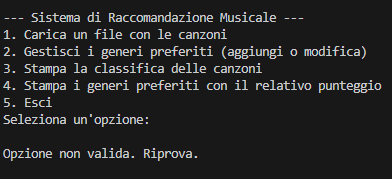
\includegraphics[width=0.5\textwidth]{htest1}
\end{center}
\begin{center}
    \textbf{Test 2}
    \par
    \vspace{0.5cm}
    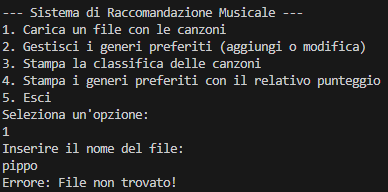
\includegraphics[width=0.5\textwidth]{htest2}
\end{center}
\begin{center}
    \textbf{Test 3}
    \par
    \vspace{0.5cm}
    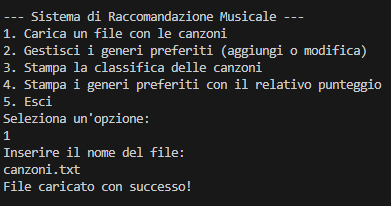
\includegraphics[width=0.5\textwidth]{htest3}
\end{center}

\newpage
\begin{center}
    \textbf{Test 4}
    \par
    \vspace{0.5cm}
    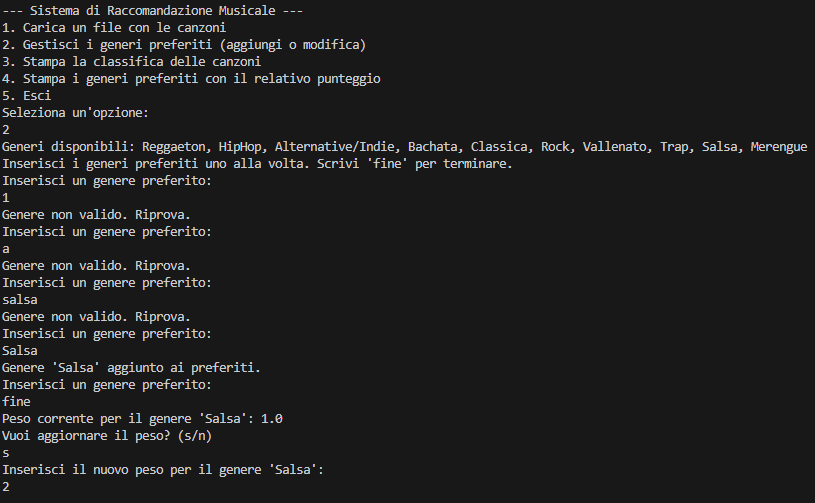
\includegraphics[width=0.5\textwidth]{htest4}
\end{center}
\begin{center}
    \textbf{Test 5}
    \par
    \vspace{0.5cm}
    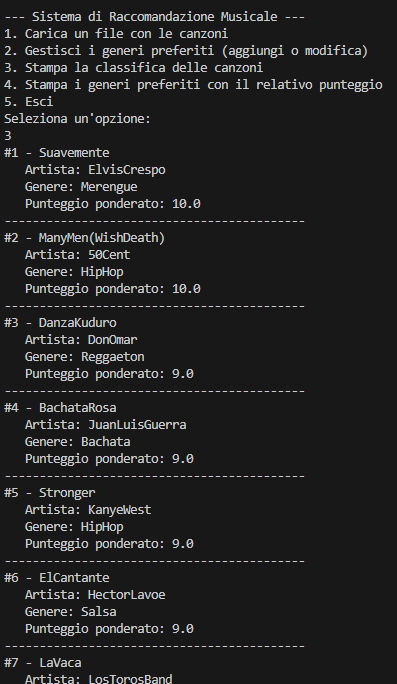
\includegraphics[width=0.5\textwidth]{htest5}
    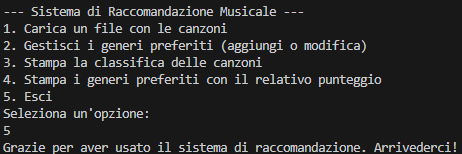
\includegraphics[width=0.5\textwidth]{htest10}
\end{center}

\newpage
\begin{center}
    \textbf{Test 6}
    \par
    \vspace{0.5cm}
    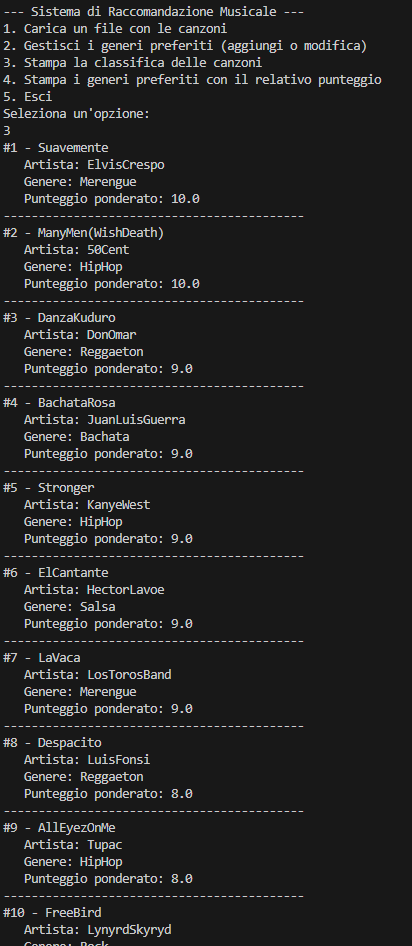
\includegraphics[width=0.5\textwidth]{htest6}
\end{center}

\newpage
\begin{center}
    \textbf{Test 7}
    \par
    \vspace{0.5cm}
    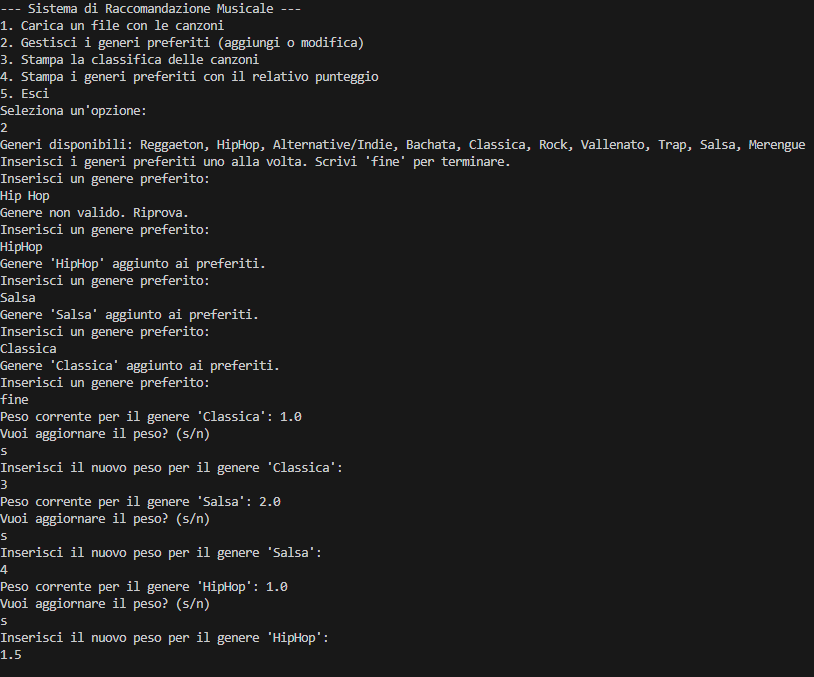
\includegraphics[width=0.5\textwidth]{htest7}
\end{center}
\begin{center}
    \textbf{Test 8}
    \par
    \vspace{0.5cm}
    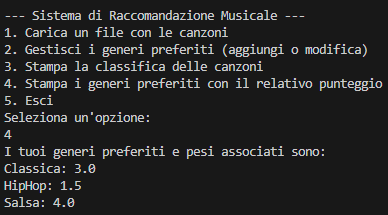
\includegraphics[width=0.5\textwidth]{htest8}
\end{center}

\newpage
\begin{center}
    \textbf{Test 9}
    \par
    \vspace{0.5cm}
    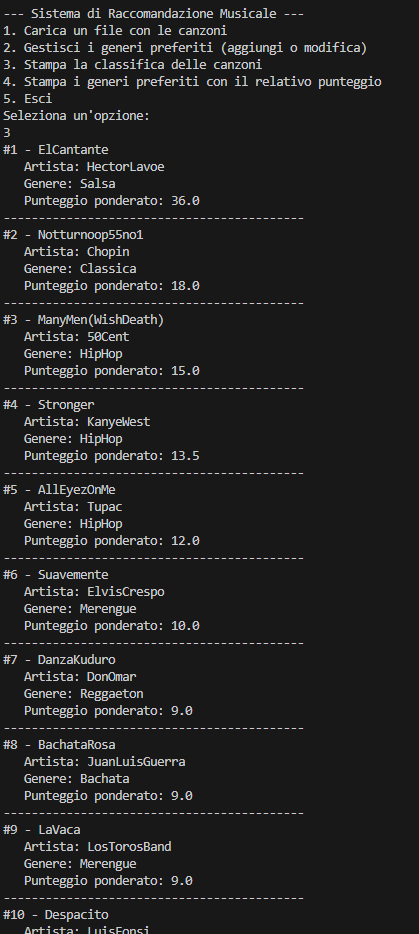
\includegraphics[width=0.5\textwidth]{htest9}
\end{center}
\begin{center}
    \textbf{Test 10}
    \par
    \vspace{0.5cm}
    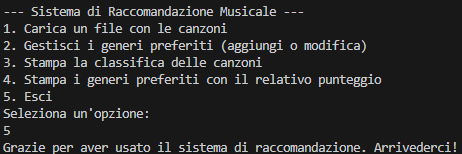
\includegraphics[width=0.5\textwidth]{htest10}
\end{center}
\vspace{1cm}

\newpage
\subsection{Testing del programma in Prolog}

\end{document}
